\documentclass[conference]{IEEEtran}

\IEEEoverridecommandlockouts                              % This command is only needed if 
                                                          % you want to use the \thanks command

\overrideIEEEmargins                                      % Needed to meet printer requirements.

% See the \addtolength command later in the file to balance the column lengths
% on the last page of the document

\usepackage{amssymb}
\setcounter{tocdepth}{3}
\usepackage{graphicx}
\usepackage[fleqn]{amsmath}
\usepackage{url}
\usepackage{amsmath} % assumes amsmath package installed
\usepackage{amssymb}  % assumes amsmath package installed
\usepackage{algorithm}			% pacchetti per i pezzi di pseudocodice
\usepackage{algorithmic}		% pacchetti per i pezzi di pseudocodice

\usepackage{float}		% pacchetto per figure e tabelle

% Lettere accentate:
\usepackage[utf8x]{inputenc}


%\usepackage{mathptmx} % assumes new font selection scheme installed
%\usepackage{times} % assumes new font selection scheme installed


% correct bad hyphenation here
\hyphenation{op-tical net-works semi-conduc-tor}


\begin{document}
%
% paper title
% can use linebreaks \\ within to get better formatting as desired
\title{SPQR@Work: Team Description Paper}

\author{\IEEEauthorblockN{Marco Imperoli, Daniele Evangelista, Valerio Sanelli, Matteo Russo, Alberto Pretto and Daniele Nardi}\\
%\IEEEauthorblockA{Department of Computer, Control, and Management Engineering\\``Antonio Ruberti``, Sapienza University of Rome, Italy.\\ Email: {\tt\small marcoimperoli@gmail.com, evangelista.1665872@studenti.uniroma1.it,\\ valerio.sanelli@gmail.com, matteo.russo@unicas.it, \{pretto,nardi\}@dis.uniroma1.it}\\
\IEEEauthorblockA{Department of Computer, Control, and Management Engineering\\``Antonio Ruberti``, Sapienza University of Rome, Italy.\\ 
Email: {\tt\small marcoimperoli@gmail.com, evangelista.1665872@studenti.uniroma1.it,}\\
{\tt\small valerio.sanelli@gmail.com, matteo.russo@unicas.it, \{pretto,nardi\}@dis.uniroma1.it}\\
Website: http://www.dis.uniroma1.it/~labrococo/SPQRWork}}


% make the title area
\maketitle

\begin{abstract}
%\boldmath
The SPQR@Work team is a spin-off of the S.P.Q.R. RoboCup team of the Department of Computer, Control, and Management Engineering “Antonio Ruberti” at Sapienza University of Rome, created to participate at the RoCKIn@Work competition.\\
This document describes the scientific background, the team members' competences and the employed robot hardware and software that the SPQR@Work team will exploit if it will be accepted to participate to the 2015 RoCKIn competition event.
\end{abstract}

\section{Introduction}
% no \IEEEPARstart
The SPQR@Work team has been founded as an offshoot of the S.P.Q.R. RoboCup team, that is involved in RoboCup competitions since 1998 in different leagues :
\begin{itemize}
\item Middle-size 1998-2002;
\item Four-legged 2000-2007;
\item Real-Rescue robots since 2003;
\item Virtual-Rescue robots since 2006;
\item Standard Platform League since 2008
 \end{itemize}

The team involves both PhD students and graduated students, members of the Cognitive Cooperating Robots laboratory, supervised by Dr. Alberto Pretto and Prof. Daniele Nardi.\\ 

SPQR@Work goals are the following:
\begin{itemize}
 \item Set up a team to successfully compete in RoCKIn@Work competition.
 \item Propose and test new techniques for (1) RGB-D object recognition and localization (2) Object manipulation and grasping (3) Robot Navigation and Planning.
 \item Promote teaching initiatives to foster the participation of students in research on intelligent mobile robotics.
\end{itemize}
 
\section{Team Presentation}
\subsection{Team Details}

\begin{itemize}
 \item \textbf{Team name:} SPQR@Work
 \item \textbf{Selected track:} RoCKIn@Work
 \item \textbf{Team members:} Daniele Evangelista, Valerio Sanelli, Matteo Russo
  \item \textbf{Team leader:} Marco Imperoli
 \item \textbf{Advisors:} Alberto Pretto, Daniele Nardi
 \item \textbf{Robot:} 1 Kuka youBot
\end{itemize}

\subsection{Involved Institutions}
\begin{figure}[t!]
\begin{center}
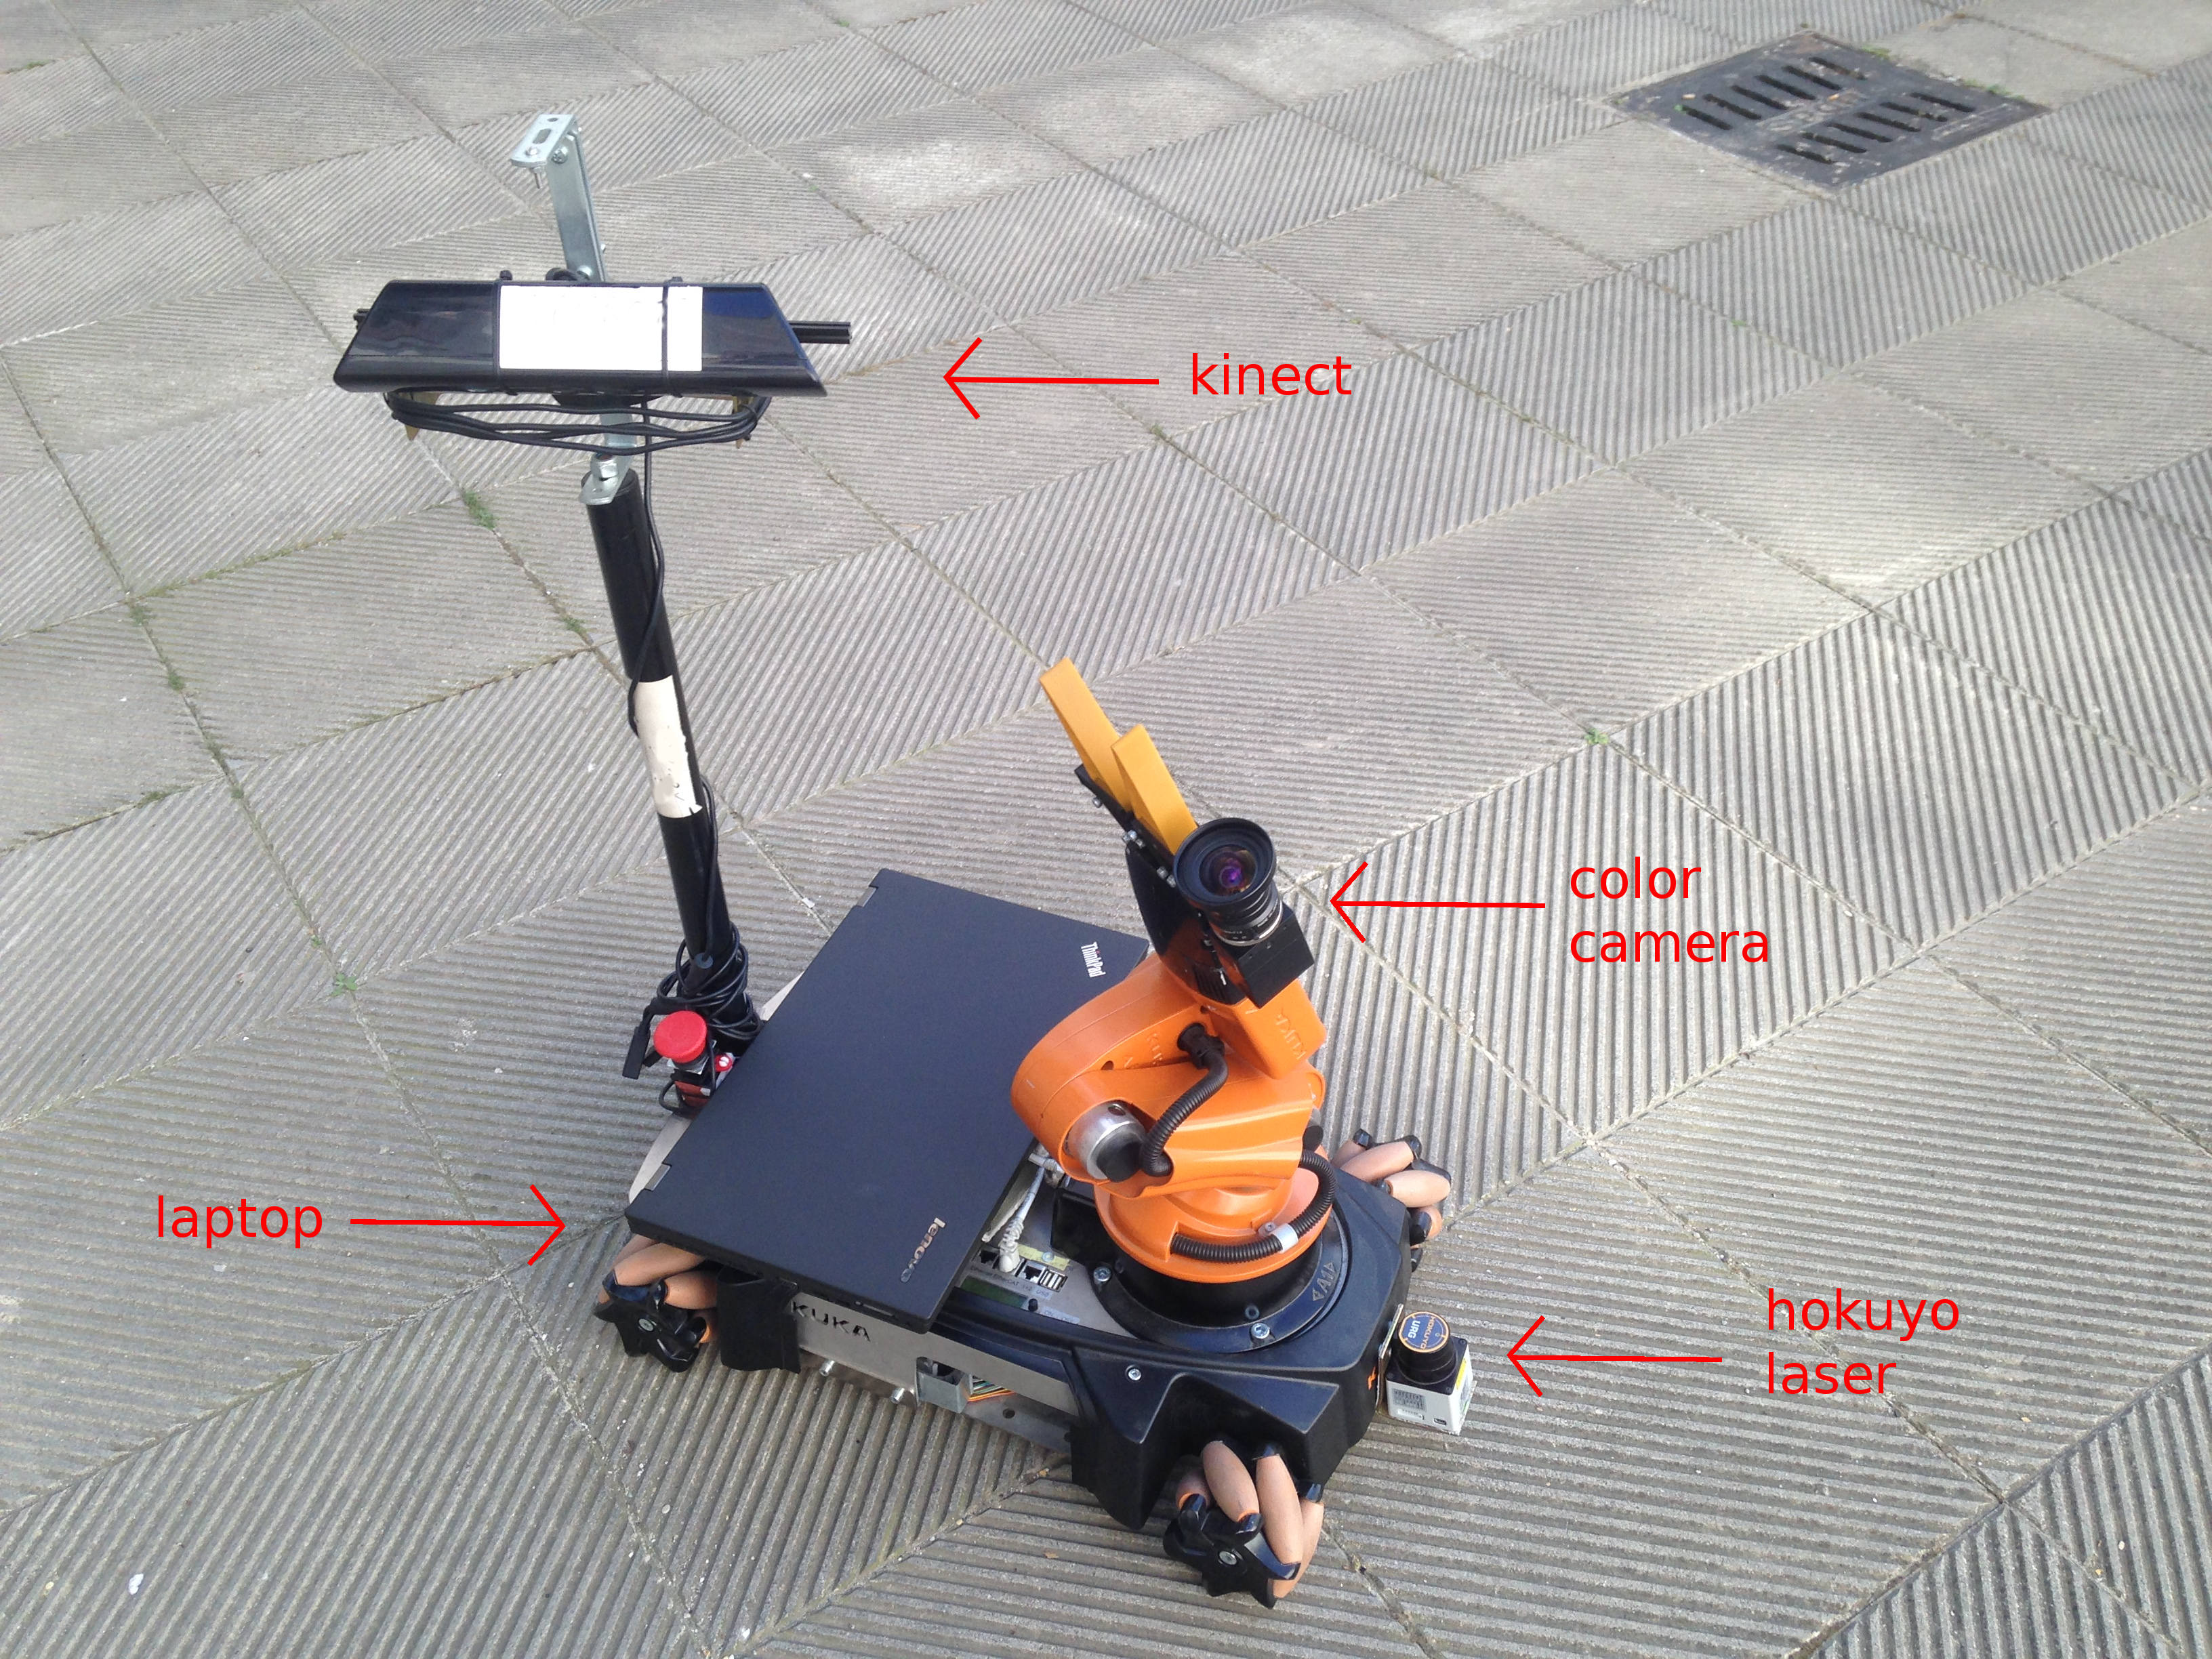
\includegraphics[width=\linewidth]{images/kuka.JPG}
\end{center}
\caption{The SPQR@Work robot}\label{fig:robot}
\end{figure}

\subsubsection{RoCoCo} The laboratory RoCoCo (Cognitive Cooperating Robots) is located at DIAG (Dipartimento di Ingegneria Informatica, Automatica e Gestionale) of Sapienza University of Rome, Italy.
The research developed at RoCoCo laboratory is in the area of Artificial Intelligence and Robotics: Lab RoCoCo has a strong background in knowledge representation and reasoning, cognitive robotics, information fusion, mapping and localization, object recognition and tracking. multi-robot coordination, robot learning, stereo-vision, vision-based people detection. RoCoCo has been involved in RoboCup competitions since 1998 in different leagues.\\

\subsection{Competence of Team Members}

\subsubsection*{Marco Imperoli}
Imperoli is a student of the Master degree in Artificial Intelligence and Robotics Engineering at Sapienza University of Rome.

\subsubsection*{Daniele Evangelista}
Evangelista is currently attending the second year of the Master degree in Articial Intelligence and Robotics at Sapienza University, in Rome. 
In October 2014 he got the bachelor degree in Informatics and Telecommunications engineering at University of Cassino. 
He is also the co-founder and CEO of \emph{alibabyte software house S.r.l.s.}, an italian company mainly focused on web, desktop and mobile 
software development. His main interests are in Machine Learning and Artificial Intelligence in robotics applications.

\subsubsection*{Valerio Sanelli}
Valerio Sanelli is a Master student of Artificial Intelligence and Robotics at la Sapienza, University of Rome.
He received the Bachelor Degree in Computer Engineering at la Sapienza in 2013.
He is mainly focused on Artificial Intelligence, with particular  emphasis on Robot Learning, Automated Reasoning and Vision systems.

\subsubsection*{Matteo Russo}
Matteo Russo is a PhD student in LARM, at University of Cassino. In September 2015 he got his M.Sc. (110/110 cum laude) in Mechanical Engineering 
at the University of Cassino, after spending 6 months at RWTH Aachen to develop his Master Thesis about robotic manipulators. 
Mechanism synthesis and analysis for robotics, industrial robots and fast prototyping are among his areas of interest.
%\subsubsection*{Roberto Capobianco}
%Capobianco received the Master Degree in Artificial Intelligence and Robotics from the Department of Computer, 
%Control and Management Engineering (DIAG) of Sapienza University of Rome. 
% During his Master's Thesis he worked in the field of Semantic Mapping, publishing a conference paper and a workshop paper on the same topic. After graduating at M.Sc. (110/110 cum laude) and successfully completing the Excellence Program, 
%After graduating, he started his Ph.D. program on November 01, 2013 at the same University. His areas of interest include robot learning, industrial and mobile robotics, and computer vision.

%\subsubsection*{Jacopo Serafin}
%Serafin obtained the Master of Science in Artificial Intelligence and Robotics from the Department of Computer, Control and Management Engineering (DIAG) of Sapienza University of Rome in March 2013. 
% Right after graduating at M.Sc.(110/110 cum laude) he has been involved in the ROVINA European project where he actually work as responsible for the 3D mapping. 
%In November 2013 he started the Ph.D. program in engineering in computer science. His areas of interest include mobile robotics, computer vision, acquisition of 3D models / maps, SLAM and least-squares estimation problems.

\subsubsection*{Alberto Pretto}

Pretto is Assistant Professor at Sapienza University of Rome since October 2013. 
He received his Ph.D. degree in October 2009 from the University of Padua, where he worked as a postdoctoral researcher at the Intelligent Autonomous Systems Lab (Department of Information Engineering). 
In 2005, he was one of the funders of IT+Robotics Srl, a spin-off company of the University of Padua working on robotics and machine vision. 
Alberto Pretto's main research activities include vision-based 3D reconstruction, visual-inertial navigation, and object recognition.

\subsubsection*{Daniele Nardi}

Nardi is Full Professor at DIS, where he was employed since 1986. His current research interests are in the field of artificial intelligence and cognitive robotics. He is Trustee of RoboCup and currently the president of the RobotCup Federation.  From 2005-2008, he also served as the co-chair of IEEE Technical Committee of International Workshop on Safety, Security and Rescue Robotics.  He is active in the context of autonomous rescue robots and successfully coordinated a team participating on several editions of RoboCup Rescue since the year 2002.  
Nardi received the ``IJCAI-91 Publisher's Prize'' and the prize ``Intelligenza Artificiale 1993'' from the Associazione Italiana per l'Intelligenza Artificiale (AI*IA).

\subsection{RoCKIn Events participations}

Imperoli and Pretto participated at the RoCKIn Camp 2014, RoCKIn Competition 2015, and RoCKIn Camp 2015, with the ``SPQR Team''. In RoCKIn Camp 2014, ``SPQR'' won in ex-aequo with another team the ``Best Practical in Perception'' award.

\section{Robot Description}

\subsection{Hardware Configuration}

The SPQR@Work robot (Fig.~\ref{fig:robot}) is a KUKA youBot with the following sensor suite:

\begin{itemize}
 \item A frontal Hokuyo laser scanner, to be used for navigation and obstacles avoidance tasks
 \item A Kinect RGB-D sensor: the area viewed by the kinect includes the working area of the arm, in order to perform object manipulation tasks without robot motions
 \item An on-board laptop running Linux Ubuntu 14.04, to be used to run \textit{all} the software modules (e.g., navigation, object recognition, etc...). The internal youBot Intel Atom PC is not used.
 \item A color USB3 high-resolution camera on the 5th joint of the manipulator for accurate object localization
\end{itemize}

The team is now actively working in improving the hardware configuration of the KUKA youBot, in particular modifications will involve both the sensors installed on the robot and
the structural layout itself.\\
A new Hokuyo laser scanner will be installed in the rear of the robot in order to improve navigation and obstacles avoidance.\\
For the object recognition and localization a new sensor will replace the current Kinect RGB-D sensor: \emph{Intel realsense f200} (https://software.intel.com/en-us/realsense/f200camera).\\
A novel gripper design is under development. A preliminary draft of this gripper is shown in Fig. \ref{fig:gripper_design}. The new mechanism is able to grasp bigger objects with a maximum finger opening equal to 135 mm. Motion is actuated by a Robotis AX-12A Servomotor, which offers higher torque when compared to the stock motor and allows for improved accuracy thanks to its embedded encoders and control. Most of the non-commercial parts of the novel design are optimized for production through 3D printing.
\\Furthermore, the layout of the KUKA youBot base platform will be enhanced in order to increase the workspace.

\begin{figure}[t!]
\begin{center}
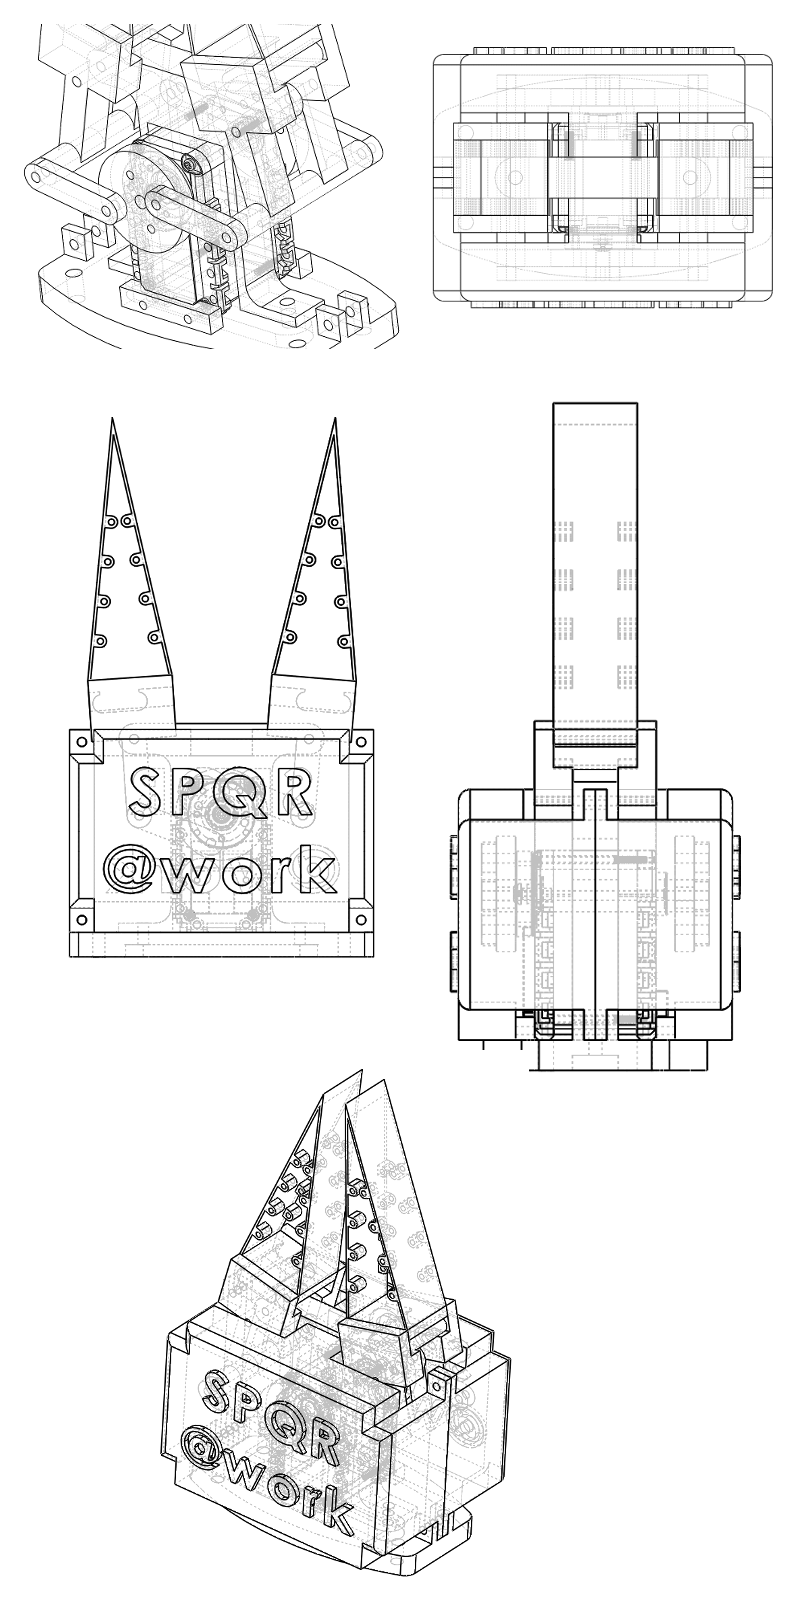
\includegraphics[angle=0,width=0.7\linewidth,]{images/gripper_design.png}
\end{center}
\caption{The new gripper design.}\label{fig:gripper_design}
\end{figure}

 
\subsection{Software Configuration}

The SPQR@Work software infrastructure is based on the ROS Indigo middleware \cite{rosweb} running on Ubuntu 14.04, nevertheless most of the developed software tools are stand-alone, middleware-agnostic: packages are integrated within ROS by means of suitable wrappers.\\
The navigation stack is based on particle filter based localization and mapping algorithms, provided by the ROS AMCL and GMapping \cite{Grisetti2007} packages, the latter implemented by one member of the laboratory RoCoCo.  Tha base motion planning task is accomplished using two different subsystems (see Fig.~\ref{fig:intro_navigation}):
\begin{itemize}
 \item A global planner, which provides the global path to follow, based on the standard MoveBase ROS package;
 \item A custom-built local planner, which, given the global plan and a costmap, produces
velocity commands to send to the mobile base controller.
\end{itemize}
Our ad hoc local planner is based on artificial potential fields, designed for holonomic mobile robots.\\

We use a custom-built module also for the manipulation and the grasping tasks: the arm motion planner we propose is able to plan accurate trajectories assuming that the best way to grasp an object disposed in an crowded environment is to let the gripper follows a straight line in the Cartesian space towards the object of interest.\\

Object recognition and localization is obtained using reliable algorithms that exploit both vision features and depth information (Sec.~\ref{sec:object_rec}). This module includes a pipeline of processing blocks (Fig.~\ref{fig:pipeline}): the pipeline includes processing blocks for sub-sampling, clustering, noise reduction, and 2D and 3D features detection and descriptors. The model matching step is performed associating the extracted features with features pre-computed from a rigid template (e.g., the CAD model) of the object. The result is a set of object candidates, that is refined using an novel object registration strategy. \\

The decision making module is based on a finite state machine implemented with the ROS Actionlib package.\\

\begin{figure*}[t!]
\begin{center}
\includegraphics[angle=0,width=\linewidth]{images/pipeline.png}
\end{center}
\caption{The SPQR@Work object recognition and localization pipeline.}\label{fig:pipeline}
\end{figure*}

Currently, the SPQR@Work robot is able to:

\begin{itemize}
 \item Localize itself and safely navigate toward a selected target area
 \item Detect QR code-like markers using vision
 \item Recognize and localize objects using RGB-D sensors, using the techniques proposed in \cite{miap_icvs2015} and \cite{prettoCASE2013}
 \item Perform simple visual-servoing and manipulation tasks (e.g., pick and place task, ``cutting a string'' task, \dots)
\end{itemize}
 
\section{Research areas and Contributions}\label{sec:research}

Several research areas are involved in the SPQR@Work team development, and some novel contributions have been proposed. Among others, a novel registration method of 3D textureless objects (Sec.~\ref{sec:object_rec}) and an arm motion planner well suited to plan
accurate trajectories also in an crowded environment (Sec.~\ref{sec:manipulation}).


\subsubsection{Object Recognition and Localization}\label{sec:object_rec}

A reliable and accurate object recognition system is an essential prerequisite to successfully compete in the RoCKIn competitions. The SPQR@Work team members presented two robust and flexible vision systems for 3D localization of untextured objects for industrial robots \cite{miap_icvs2015, prettoCASE2013}. In particular, in \cite{miap_icvs2015} we presented a robust and efficient method for object detection and 3D pose estimation that exploits a novel edge-based registration algorithm we called Direct Directional Chamfer Optimization (D\textsuperscript{2}CO). D\textsuperscript{2}CO refines the object position employing a non-linear optimization procedure, where the cost being minimized is extracted directly from a 3D image tensor composed by a sequence of distance maps. No ICP-like iterative re-association steps are required: the data association is implicitly optimized while inferring the object pose. Our approach is able to handle textureless and partially occluded objects and does not require any off-line object learning step: just a 3D CAD model is needed (see Fig.~\ref{fig:obj_model}).

\begin{figure}[t!]
\begin{center}
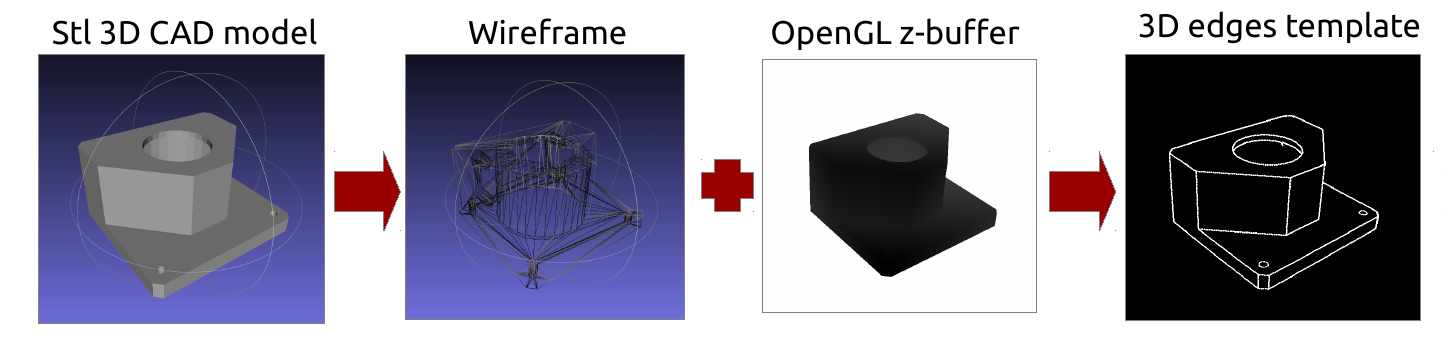
\includegraphics[angle=0,width=\linewidth]{images/d2co_00.png}
\end{center}
\caption{The raster models used in our algorithms are computed from the 3D CAD models of the objects.}\label{fig:obj_model}
\end{figure}
The Directional Chamfer Distance (DCD) tensor encodes the minimum distance of an image point to an edge point in a joint direction/location space. Unlike the Chamfer distance, the DCD takes into account also the edges directions (see Fig.~\ref{fig:tensor}).

\begin{figure}[t!]
\begin{center}
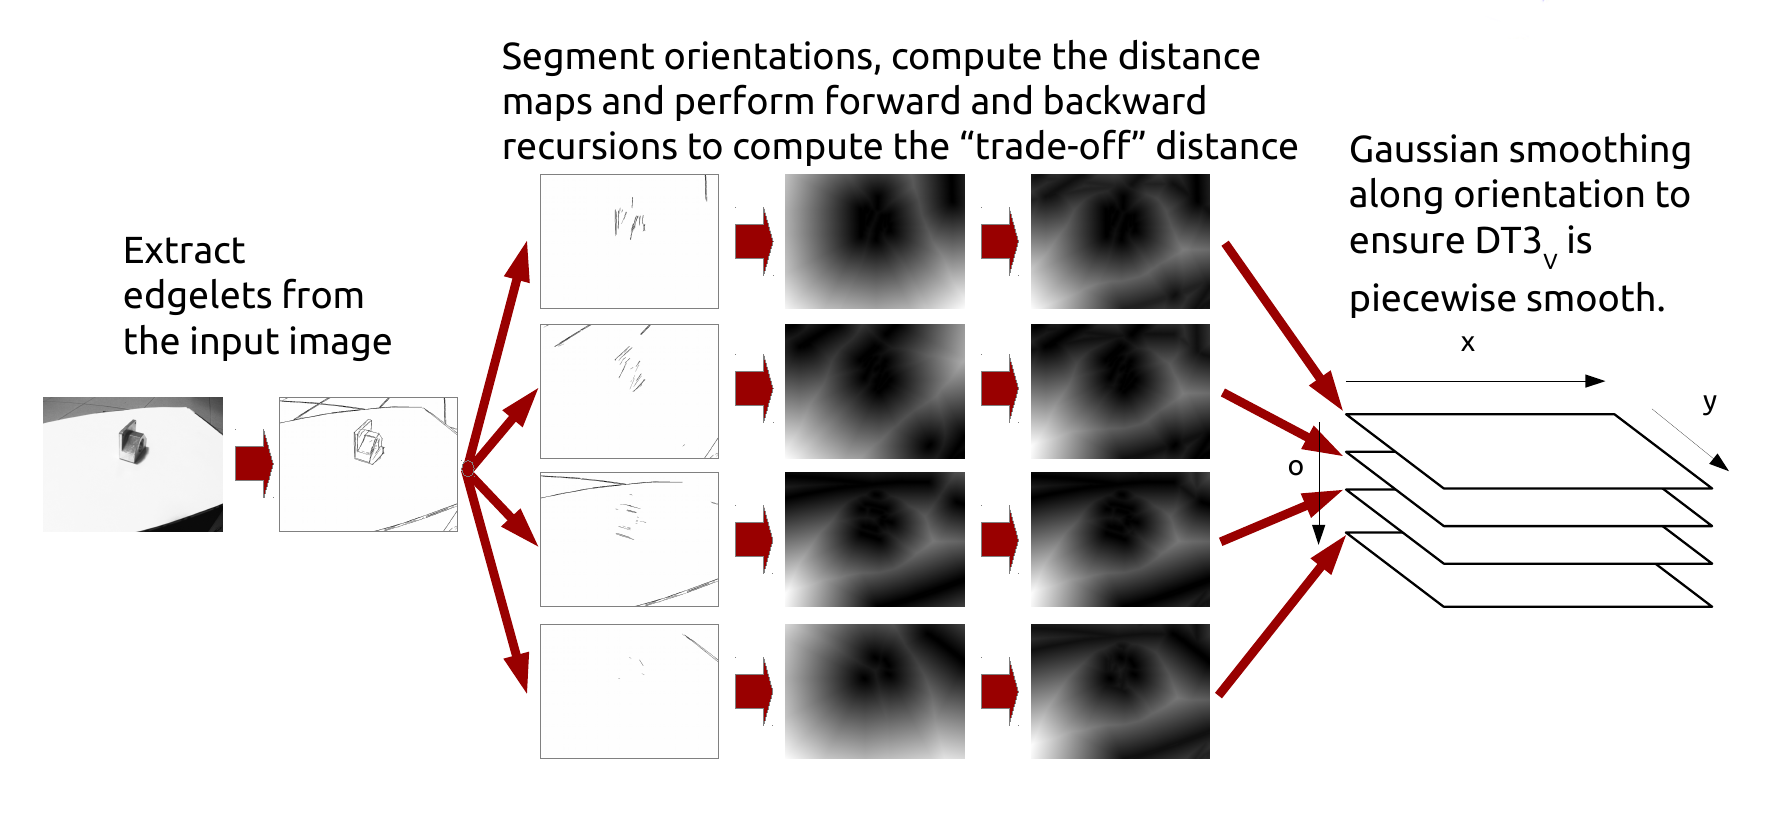
\includegraphics[angle=0,width=\linewidth]{images/d2co_01.png}
\end{center}
\caption{DCD tensor computation pipeline.}\label{fig:tensor}
\end{figure}

We extract a set of object candidates by pre-computing the (projected) raster templates along with their image orientations for a large number of possible 3D locations; for each point, we lookup the DCD tensor, computing the template average distance. The templates are then sorted for increasing distances.\\

D\textsuperscript{2}CO finally refines the object position employing a non-linear optimization procedure that minimizes a tensor-based cost function (e.g., see Fig.~\ref{fig:sample_d2co}). We use the LM algorithm with a Huber loss function in order to reduces the influence of outliers. During the optimization, both the (projected) points position and the (projected) points orientation are constantly updated.

\begin{figure}[t!]
\begin{center}
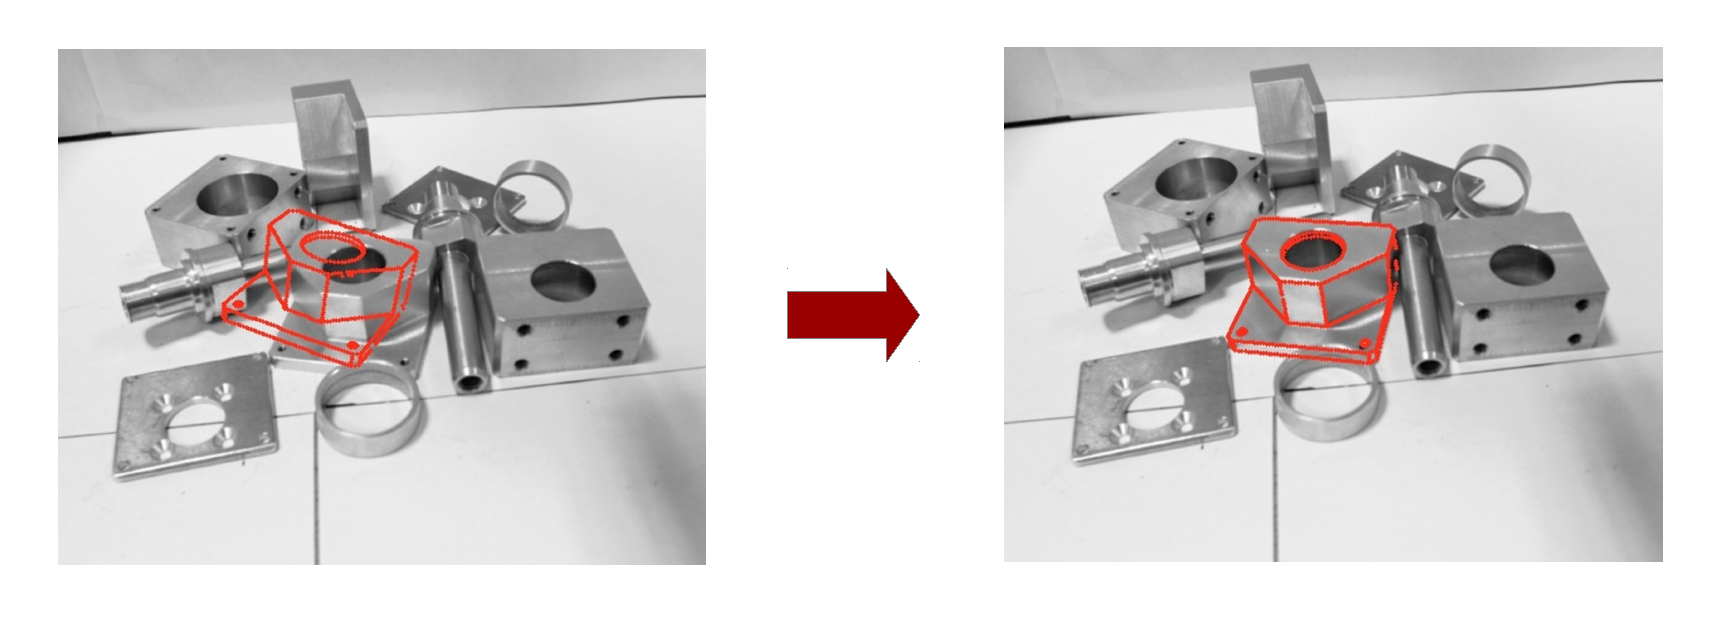
\includegraphics[angle=0,width=\linewidth]{images/d2co_02.png}
\end{center}
\caption{An example of object registration using the D\textsuperscript{2}CO algorithm.}\label{fig:sample_d2co}
\end{figure}

\subsubsection{Object Manipulation and Grasping}\label{sec:manipulation}

Very often, the objects to be manipulated are randomly disposed in cluttered environments: a precise, smooth and safe arm trajectory planning is an essential requirement. The arm motion planner we propose is able to plan accurate trajectories assuming that the best way to grasp an object disposed in an crowded environment is to let the gripper follows a straight line in the Cartesian space towards the object of interest. Thanks to our obstacles avoidance system, each planned path is guaranteed to be free from collisions, and very accurate object grasping and placing are performed. In order to accomplish the manipulation task, we have defined a set of arm control points along with two different obstacles representations: spherical and box obstacles (e.g., see Fig.~\ref{fig:intro_manipulation}). Using these primitives, our trajectory planner can easily compute collision-free paths. 

\begin{figure}[h!]
\begin{center}
\begin{minipage}[b]{0.32\linewidth}
	\begin{center}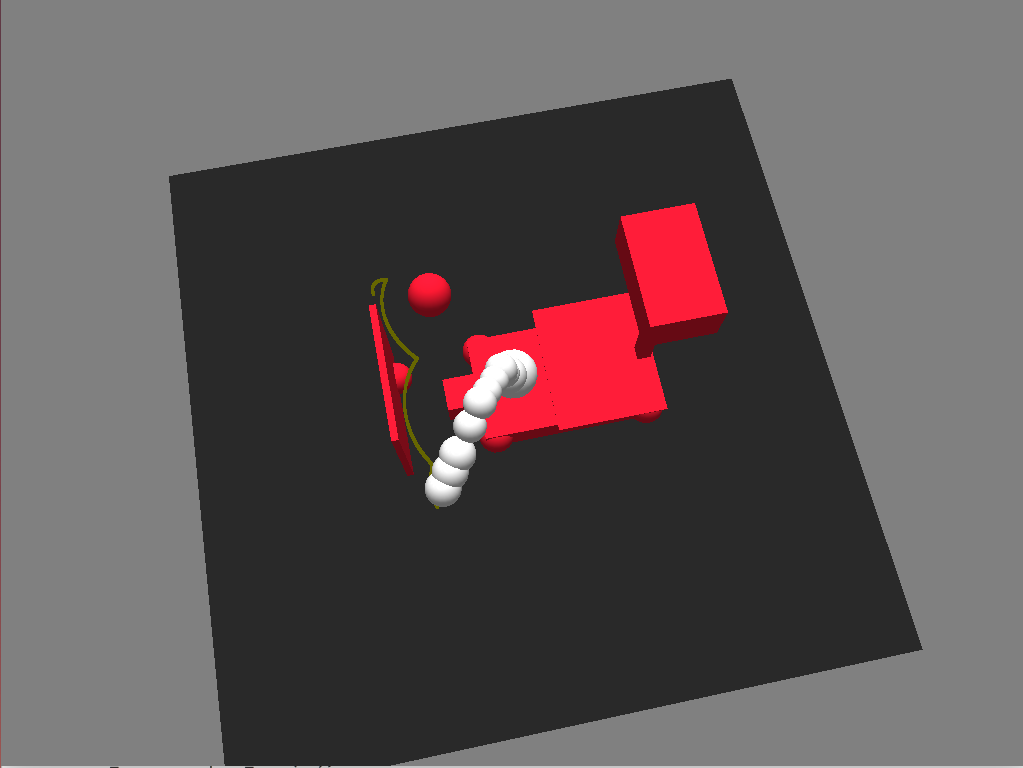
\includegraphics[angle=0,width=\linewidth]{images/av7.png}\end{center}
\end{minipage}\hfill
\begin{minipage}[b]{0.32\linewidth}
	\begin{center}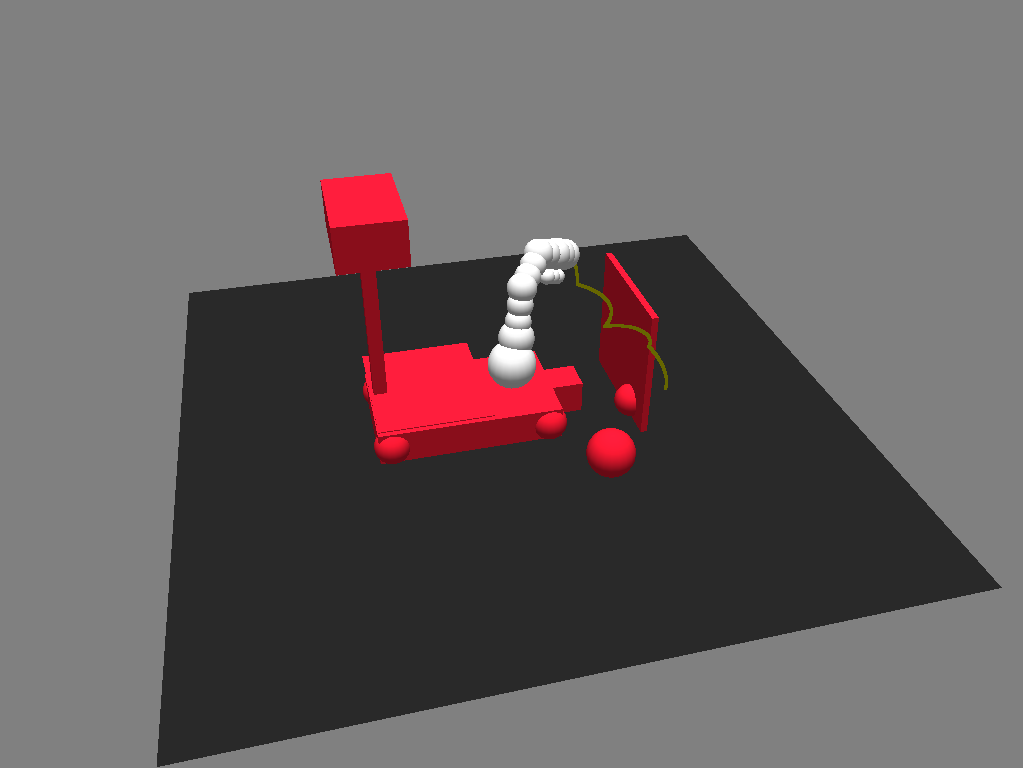
\includegraphics[angle=0,width=\linewidth]{images/av8.png}\end{center}
\end{minipage}\hfill
\begin{minipage}[b]{0.32\linewidth}
	\begin{center}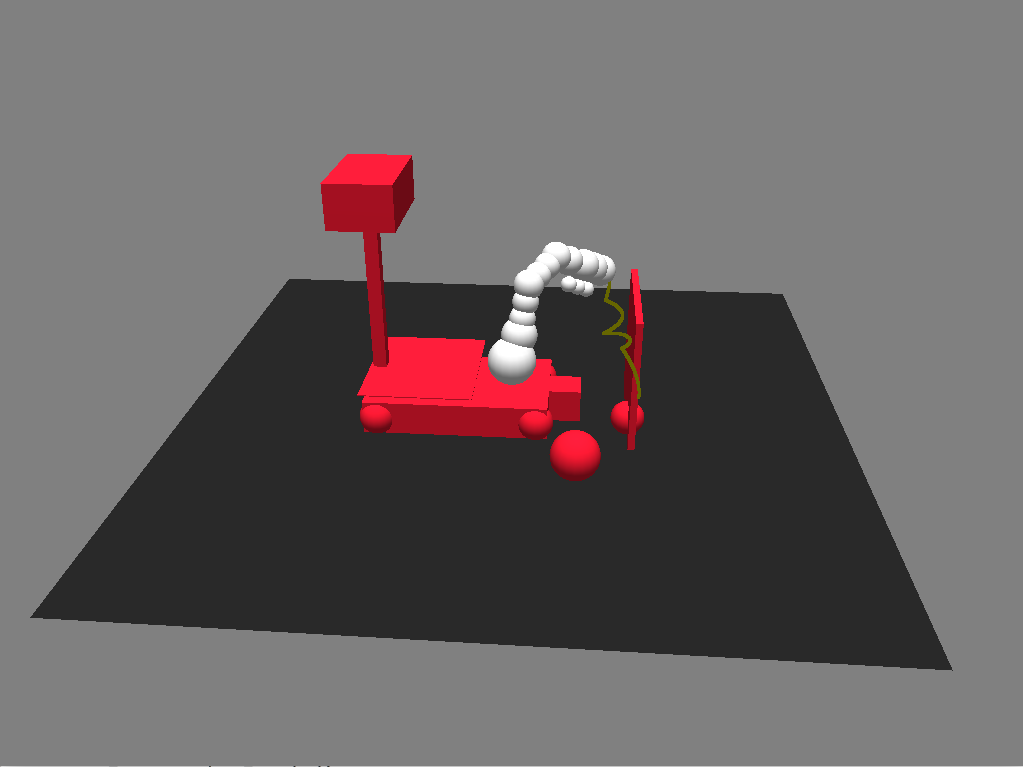
\includegraphics[angle=0,width=\linewidth]{images/av9.png}\end{center}
\end{minipage}\hfill
\end{center}
\caption{Visualization of three different points of view of the same scene using our OpenGL GUI. The manipulator control points and the obstacles are rendered in white and red respectively. The yellow path represents the planned end-effector trajectory. }\label{fig:intro_manipulation}
\end{figure}


\subsubsection{Robot Navigation and Planning}\label{sec:navigation}


In our experience, we found that the existing navigation frameworks (e.g., the popular ``move\_base'' package of the ROS framework \cite{rosweb}) usually depends on a large number of parameters: it is usually very difficult to find a good parameters set that enables a reliable and safe navigation in most of the conditions. To address this problem, we developed an ad hoc \textit{local} planner based on artificial potential fields, designed for holonomic mobile robots. The idea is to use an existing navigation framework as a primary navigation system, focusing on the planning reliability and safety. Our local planner is then used only for refinement purposes, improving the accuracy (see Fig.~\ref{fig:intro_navigation}).

\begin{figure}[h!]
\begin{center}
\begin{minipage}[b]{0.6\linewidth}
	\begin{center}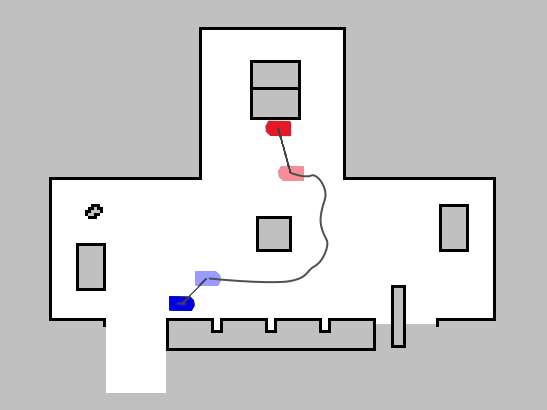
\includegraphics[angle=0,width=\linewidth]{images/navigation.png}\end{center}
\end{minipage}\hfill
\end{center}
\caption{An example of navigation path (dark gray). The curved portion of the entire path is computed by the primary navigation planner. Our potential fields based planner is used for approaching the final target (red) and for sliding away from obstacles at the beginning of the navigation task (blue).}\label{fig:intro_navigation}
\end{figure}

Moreover, in order to improve the whole navigation system, we adopt a robot odometry refinement technique, that allows to enhance the robot localization accuracy. This method performs a fast matching between the incoming laser scans. The robot odometry is then updated according with the displacement computed by a scan matcher.\\

\section{Reusability and Relevance to Industrial Robotics}

\begin{itemize}
 \item Some modules of the proposed object recognition and localization systems (Sec.~\ref{sec:object_rec}) is currently installed in seven real world industrial plants \footnote{E.g., https://www.youtube.com/watch?v=jqhuEjnDdfI}, with different setups, working with hundreds of different models and successfully guiding the manipulators to pick several hundreds of thousands of pieces per year. 
 \item Our current arm trajectory planning and control system rivals other state-of-the-art planning frameworks (e.g., MoveIt! \cite{moveitweb}). We aim to further improve this module and possibly to make it publicly available.
\end{itemize}

\bibliographystyle{IEEEtran}
\bibliography{bibliography} 

% that's all folks
\end{document}
